\chapter{Model description, data and analysis method} 
In this thesis the dust emission model 
FLEXDUST\footnote{\url{https://git.nilu.no/christine/flexdust/-/tree/b07dc58226a3e0844328482d343ab6a14f3869c7} (last access 06/05/2021)} 
\parencite{flexdust_ref_2016} and the Lagrangian particle dispersion model 
FLEXPART\footnote{ \url{https://git.nilu.no/flexpart/flexpart/-/tree/release-10.4.1} (last access 06/05/2021)} 
\parencite{Flexpart10.4_ref} was used to 
simulate the spring time dust deposition between 1999 and 2019 at 7 sites across the Chinese Loess Plateau. Both FLEXDUST and FLEXPART are developed at the Norwegian Institute for air research (NILU). 

\textcite{flexdust_ref_2016} used the same two models to study the transport and deposition of high latitude dust, where they simulated the dust transport from a source oriented viewpoint, following the dust from the source to deposition. Here the dust transport and deposition is simulated from a receptor viewpoint, where all the dust that could possibly be deposited at receptor location are tracked backward in time to probe for a possible sources. The distribution of source possibilities are then constrained by the emission field produced by FLEXDUST. The modelling workflow is summarised by the flow chart in \Cref{fig: flow_chart}. 

\begin{figure}[!ht]
  \centering
\begin{tikzpicture}[thick,node distance=2cm, scale=0.6, every node/.style={scale=0.8}]
    \node (start) [startstop, align=center] {\Large \verb|Flex_extract| \\Data retrieval from ECWMF servers};
    \node (in1) [io, below of=start, align=center] {ERA5 input fields \\ 3hourly, \ang{0.3} $\times$ \ang{0.3}};
    \node (flexpart) [process, below right=0.6cm and 0.8cm of in1, align=center] {\Large \verb|FLEXPART| \\ Dust transport and deposition, \\ backward simulations starting from \\ the specified receptor location.};
    \node (flexdust) [process, below left=1cm and 0.8cm of in1, align=center] {\Large \verb|FLEXDUST|};
    \node (emssens_wetdep) [io, below of=flexpart, align=center, xshift=60, node distance=2.5cm] {Wet deposition \\ sensitivity };
    \node (emssens_drydep) [io, below of=flexpart, align=center, xshift=-70, node distance=2.5cm] {Dry deposition \\ sensitivity};
    \node (dust_emissions) [io, below of=flexdust, align=center, node distance=2.9cm] {Dust emission flux \\ \si{\kg\per\square\metre}};
    \node (pprocess) [process, below of=start, align=center, node distance=10cm] {\Large Post processing \\ Emissions sensitivities are multiplied \\ with corresponding dust emissions.};
    \node (source_contrib) [io, below of=pprocess, align=center, node distance=3.5cm, xshift=-50] {\Large Source contribution \\ i.e. how much each source \\ element is contributing to \\ dry and wet deposition at \\ the receptor.};
    \node (stop) [startstop, right of= source_contrib,align=center,  node distance=9cm] {\Large Dust deposition at \\ \Large the receptor \\ the total contribution \\ from all source elements.};
    \draw [arrow] (start) -- (in1);
    \draw [arrow] (in1) -| (flexpart);
    \draw [arrow] (in1) -| (flexdust);
    \draw [arrow] (flexpart) -- (emssens_wetdep);
    \draw [arrow] (flexpart) -- (emssens_drydep);
    \draw [arrow] (flexdust) -- (dust_emissions);
    \draw [arrow] (emssens_wetdep) |- (pprocess);
    \draw [arrow] (dust_emissions) -- (pprocess);
    \draw [arrow] (emssens_drydep) -- (pprocess);
    \draw [arrow] (pprocess) -- (source_contrib);
    \draw [arrow] (source_contrib) -- (stop);
\end{tikzpicture}
\caption{Flow chart showing the workflow for the modelling analysis. }
\label{fig: flow_chart}
\end{figure}

The receptor oriented backwards simulation approach was chosen over the forward approach due to being more computationally efficient when the number of source elements greatly exceed the number of receptors. In addition the backward approach allow to naturally deal with point receptors, whereas in a forward simulation the deposition at the receptor location has to be interpolated from the model output grid. The backward approach also makes it possible to determine exactly which source regions that are contributing to deposition at receptor.     

Compared to conventional integrated dust models, the Largrangian modelling framework used in FLEXPART does not require a computational grid. This means that Lagrangian models to are almost devoid of artificial numerical diffusion, and the only errors are due to interpolation of meteorological variables to the particle position and the in discretisation of the differential equation. The limited amount of numerical diffusion allow FLEXPART better preserve filament structures within the dust plume that in a Eulerian model would be smoothed out \parencite{cassiani_offline_2016}. However a limitation with FLEXPART and FLEXDUST is that they are completely depended on the quality and amount information available in input data, this constrains the complexity of the parameterizations that can be implemented \parencite{flexpart_wetdep}. Whereas in an online Eulerian dust model any variable required can be calculate by the model it self.       

The simulations have been conducted on the Saga super computer operated by the Norwegian high performace 
computing center, Sigma2. For storage and post analysis, the data is transferred to the 
NIRD computing infrastructure (National Infrastructure for Research Data). 


\section{Flex\_extract}
Both FLEXPART and FLEXDUST depend on external meteorological input data. \verb|Flex_extract| is a package developed to retrieve and prepare the necessary meteorological input data from the European Centre for Medium weather forecast (ECWMF) servers for running FLEXPART simulations \parencite{tipka_flex_extract_2020}. 
The version of \verb|flex_extract| used here was 7.0.4, to retrieve the necessary input field from ERA5 reanalysis at 3hourly temporal resolution at $0.3\degree \times 0.3\degree$ spatial resolution for the region of East asia from March until May for the years from 1999 to 2019. The retrieval process can be rather slow as a large amount of data needs to be downloaded.     

\subsubsection{ERA5}
ERA5 is the latest reanalysis produced by the ECWMF. 
The ERA5 reanalysis assimilate large amount of observational data in order to provide the best estimate of the state of the atmosphere extending back to 1979 \parencite{hersbach_era5_2020}. Compared to its predecessor ERA-Interim, ERA5 offers higher spatial resolution of $0.25\degree \times 0.25\degree$, with up to hourly temporal resolution, and is based on a more recent version of the integrated forecast system (IFS). 

\section{FLEXDUST}\label{sec:flexdust}
FLEXDUST is a global dust emission model, specifically developed to be used together 
with FLEXPART for studying long range dust transport and deposition. FLEXDUST relies on common 
formulations for dust emissions found in global climate models \parencite{flexdust_ref_2016}. FLEXDUST is a bulk emission scheme as decribed in \Cref{sec:dust_emission_modelling}. 

A crucial part of any dust emission model is to identify the regions with high bare soil 
fraction, which are regions that are likely exposed to wind erosion. FLEXDUST utilise the satellite 
based Global Land Cover map version 3, by National Mapping Organisations (GLCNMO) with at 
resolution of 15 arcseconds \parencite{shirahata2017production} to obtain the bare soil fraction globally.
In addition to bare soil regions, FLEXDUST also considers partly vegetated areas as possible
dust sources. The available soil fraction for partly vegetated areas are determined by
subtracting the vegetation cover included from the ECWMF meteorological forcing.
Depressions are often more favourable to dust emissions as sediments are more easily gathered there \parencite{zender2003mineral}. Therefore FLEXDUST apply the erodibility scaling 
\Cref{eq_ero_soil_frac} according to \textcite{dust_dist_Ginoux2001}. 
\begin{equation}\label{eq_ero_soil_frac}
    S = \left(\frac{z_{max} - z_i}{z_{max} - z_{min}}\right)^5 
\end{equation}    
Here $z_i$ is the local elevation and $z_{max}$ and $z_{min}$ is the minimum and
maximum elevation in a 10\degree $\times$ 10\degree area.  The erodibility $S$ is
then scaled by the bare soil fraction to get the erodible soil fraction. The erodible soil fraction over East Asia is shown in \Cref{fig:erodible_soil_fraction_EA}. 
\begin{figure}[hptb]
    \centering
    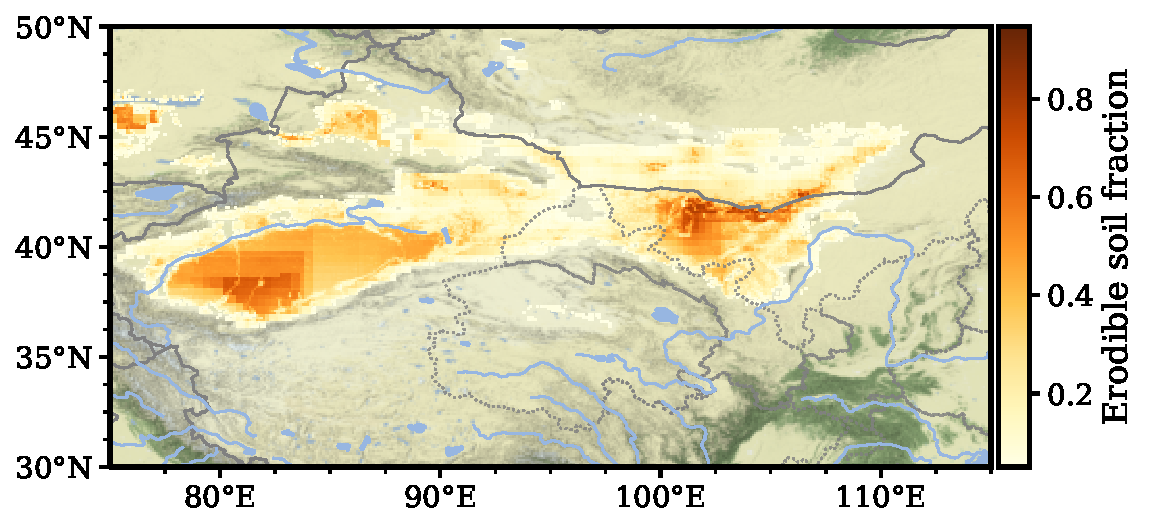
\includegraphics[width=\textwidth]{../figs/erodible_soil_fraction.pdf}
    \caption{The erodible soil fraction from FLEXDUST over the East Asia}
    \label{fig:erodible_soil_fraction_EA}
\end{figure}

In FLEXDUST dust emission occur when the friction velocity exceeds the minimal threshold 
friction velocity of the particles in the soil bed. Based on wind tunnel experiments, dust 
particles with equivalent diameter between \SI{75}{\micro\metre} - \SI{100}{\micro\metre} has 
the smallest threshold friction velocity (\cref{fig:treshold_friction_velocity_ps}). The 
threshold friction velocity $u_{*t0}(d)$ in FLEXDUST is determined by the 
\SI{75}{\micro\metre} particles, following the idealised expression of \textcite{shao2000simple}:
\begin{equation}
    u_{*t0}(d) = \sqrt{a_1 \left(\frac{\rho_p}{\rho_a}gd+\frac{a_2}{\rho_ad}\right)} 
\end{equation}
Here $a_1$ and the scaling constant for the inter particle forces, $a_2$  is assumed to be 0.0123 and \SI{3.0}{\kg\per\s\squared} respectively, which is  
according to \textcite{shao2000simple}, $\rho_p$ is the particle density and $\rho_a$ is the air density. 
For regions where there are clay and silt present, but no sand, \SI{10}{\micro\metre} 
particles are set to determine the threshold friction velocity. In FLEXDUST clay and 
silt fractions can either be obtained from ISRIC 250m resolution Soil Grids dataset 
\parencite{soil-grid_ref} or from the Global soil Data \cite{task2014global} dataset. 

The effect of soil moisture on the threshold friction velocity is parametrized according to \textcite{fecan1998parametrization}:
\begin{equation}
    \begin{cases}
    \frac{u_{*tw}}{u_{*t}}=1, & \text{if } w < w' \\
    \frac{u_{*tw}}{u_{*t}}=\sqrt{1+1.21(w-w')^{0.68}}, & w \geq w'
    \end{cases}
\end{equation}
where $w$ is the volumetric water content of the soil (\%). If the soil moisture exceed $w'$, the capillary 
forces will start affecting the threshold friction velocity. Where $w'$ is given by \Cref{eq:moisture_clay} 
and depends on the clay content $c$ (\%).   
\begin{equation} \label{eq:moisture_clay}
    w' = 0.17c + 0.0014c^2
\end{equation}
The soil moisture content is retrieved from the ECWMF input fields. Further, snow cover is 
assumed to inhibit dust emissions and snow cover data is also obtained from the ECWMF input fields. 
\par In partly vegetated areas non-erodible surface elements would increase the surface 
roughness affecting the dust emissions. In FLEXDUST the drag partition to non-erodible 
surface elements for partly vegetated areas are accounted for following the description in 
\parencite{zender2003mineral}, by scaling the mobilisation threshold by $f_d$ according to \Cref{eq:drag_partition}:
\begin{equation}\label{eq:drag_partition}
    f_d = \left[1 - \frac{\ln (z_{0m}/z_{0s})}{0.35\ln (0.1/z_{0s})^{0.8}}\right]^{-1}
\end{equation}
Here $z_{0m}$ is the roughness length of momentum transfer and $z_{0s}$ is the smooth roughness length which 
describe roughness of a bed of potentially erodible particles without any non erodible elements. Wind tunnel 
experiments has shown that: 
\begin{equation}
    z_{0s} \approx D/30
\end{equation}
where $D$ is the particle diameter. In FLEXDUST it is assumed globally uniform values of  $z_{0m}=\SI{100.0}{\micro\metre}$ and $z_{0s}=\SI{33.3}{\micro\metre}$

After the mobilisation threshold is calculated,  the dust emissions flux is derived following the paremeterisation of the vertical dust flux as described in \textcite{MB95_dust_emission}: 
\begin{equation}
    F=c\alpha \frac{\rho u_{*}^3}{g}\left(1-\frac{u^2_{*t}}{u^2_*}\right)\left(1+ \frac{u_{*t}}{u_*}\right)
\end{equation}
where $u_*$ is the friction velocity, c is a constant scaling factor ($4.8\cdot 10^{-4}$) and $\alpha$ is the sand blasting efficiency:
\begin{equation}\label{eq:sand_blasing_eff}
    \alpha = 100\exp{(13.4f_{clay}-6)\ln 10}
\end{equation}
\Cref{eq:sand_blasing_eff} is only valid for clay fraction $\leq$ 0.2, so if the clay fraction exceed 0.2 it is set to 0.2 in FLEXDUST \parencite{zender2003mineral}. 



The small dust particles (< \SI{20}{\micro\metre}) has a greater potential to experience long range transport due their smaller settling velocities. Since FLEXDUST was developed with the purpose of studying long range dust transport, the emitted dust is assumed to have a volume size distribution varying between \SI{0.2}{\micro\metre} and \SI{18.2}{\micro\metre}. This size distribution is based on brittle fragmentation theory described in \textcite{kok_scaling_2011}. The log normal volume size distribution is determined according to \Cref{eq:size_dist}. 

\begin{equation}\label{eq:size_dist}
    \frac{\text{d} V_d}{\text{d} \ln D_d} = \frac{D_d}{c_v}\left[1 + \text{erf}\left(\frac{\ln(D_d/\overline{D_s})}{\sqrt{2}\ln \sigma_s}\right)\right]\text{exp}\left[-\left(\frac{D_d}{\lambda}\right)^3\right]
\end{equation}
Where $c_v = \SI{12.62}{\micro\metre}$ is a normalisation constant, $\overline{D_s}=\SI{3.4}{\micro\metre}$ and $\sigma_s = 3.0$ is the median diameter and the geometric standard deviation respectively.  

\section{The Lagrangian particle dispersion model: FLEXPART}

\par The dust transport and deposition is calculated by FLEXPART (Flexible Particle dispersion model). FLEXPART is an offline Lagrangian particle dispersion model (LPDM), that has been been to applied to study transport of a wide range of atmospheric atmospheric tracers, eg. mineral dust, black carbon and volcanic ash \parencite{flexdust_ref_2016,choi_investigation_2020, eckhardt2008estimation}. FLEXPART is driven by 3-hourly ERA5 meteorological reanalysis at $0.3\degree \times 0.3\degree$ spatial resolution. The version of FLEXPART used is 10.4 which includes the improved wet deposition scheme based on cloud information from the ECWMF input fields \parencite{flexpart_wetdep}. 
\par FLEXPART calculates trajectories for a large number computational particles (from here on referred to as particle and not be confused with real dust particles) that follow the wind-fields resolved in the meteorological input data with parameterizations of the turbulent motions, subgrid-scale convection, and gravitational settling imposed on the trajectories. Each particle represent a dust-aerosol population with a log-normal mass size distribution with a specified density and mean particle diameter. In addition ice nucleation efficiency ,$IN_{eff}$, cloud condensation nuclei efficiency $CCN_{eff}$ and efficiency of below cloud scavenging by rain $C_{rain}$ and snow $C_{snow}$, can be assigned to the particle regulating the strength of the wet deposition in the model.   

FLEXPART can be either run forward in time from the source to receptor, or backwards from the receptor to the source. The main distinction between forward and backward simulations, is in how the emission strength is constrained. In a forward simulation particles are released at the source and the emitted mass which the particles carry are defined prior to the particle release directly yielding the concentration and deposition on a regular longitude latitude at each time step. 

However in a backward simulation the particle release happens at the receptor and the emission strength is unknown. Then the purpose of the particles in a backward simulation is to probe for the possible source regions and establish the emission sensitivity i.e. how sensitive the deposition at receptor would be to a potential source element. The final output correspond to a distribution of possible source areas at each time step also called emission sensitivity. The emission sensitivity is constructed in such that when multiplied by the emission flux with units \si{\kg\per\cubic\metre\per\s} would produce a map of how much each source element are contributing to the concentration or deposition at the receptor.  

For backward simulation the concentration, wet and dry deposition has to be obtained in separate simulations, due  the manner in which the particles are released depends on the configuration.  
\subsection{FLEXPART: dry deposition}
In the atmosphere the dry deposition flux vary with height. In the boundary layer turbulent diffusion and gravitational settling are dominating and close to the surface in the quasi-laminar sublayer brownian motion and gravitational settling dominate. 

In FLEXPART the dry deposition is represented by calculating the dry deposition velocity $v_d(z)$, and when multiplied with the concentration at a specified height yields the deposition flux. The last stage of deposition from the air to the surface is quite complex and depend both on the properties of the surface and the dust particle it self. 
FLEXPART includes both a dry deposition scheme for particulate matter as well as gasses, and is calculated according to a two layer resistance model \parencite{Flexpart-2005_ref_paper}. For particulate matter the deposition velocity is calculated according to:
\begin{equation}
    v_d=[r_a + r_b + r_a r_b v_g]^{-1} + v_g
\end{equation}
where $r_a$ is the aerodynamic resistance, $r_b$ is the quasi laminar surface layer resistance ,$v_g$ is the settling velocity and the product $r_a r_b v_g$ represent a virtual resistance \parencite{GIARDINA201811_drydepo}. The gravitational settling velocity is calculated according to \textcite{slinn1982predictions}:
\begin{equation}
    v_g = \frac{g\rho_p d_p^2 C_{cun}}{18\mu}
\end{equation}
where $\rho_p$ and $d_p$ is the particle density and diameter, $\mu$ is the dynamic viscosity of air and $C_{cun}$ is the Cunningham slip-flow correction.

In backward mode dry deposition is calculated at start of the simulation by releasing the particles in a shallow layer close to the ground. This layer corresponds to the layer which particles in forward mode would be subjected to dry deposition and by default is set to 30m. The "mass" of the particles are then scaled by the deposition velocity and tracked backward in time as in regular backward simulation \parencite{eckhardt2017source}. 

\subsection{FLEXPART wet deposition}

The wet deposition scheme in FLEXPART was recently improved in \textcite{flexpart_wetdep}, to take advantage of cloud information recently available from the ECWMF forcing. The the wet deposition scheme in FLEXPART consist of two steps. First the location of the particle in relation to the cloud is determined using the 3D specific cloud total
water content (CTWC).  Then based on the particle's location in relation to the cloud, the particle can either be subjected to nucleation scavenging inside the cloud, or impaction scavenging below the cloud. If the particle is above the cloud no scavenging can occur. 

In backward mode the wet deposition is calculated before the particle. Since wet deposition can occur throughout the whole atmospheric column, the particles are released over the whole atmospheric column to check if any particles are subjected to wet deposition. FLEXPART then calculates the trajectories for wet deposited particles starting at the height where the particles were scavenged and the remaining particles are terminated.    
\subsubsection{In cloud scavenging}
The in-cloud scavenging scheme in FLEXPART is only activated for particles residing within a precipitating cloud. Precipitation does not necessarily occur over the whole grid cell in the input data, accordingly FLEXPART uses an empirical relation to derive the fraction of a gridcell experiencing precipitation , see \textcite{Flexpart-2005_ref_paper} for details. The subgrid precipitating cloud water (PCW) is calculated according to: 
\begin{equation}
    PCW = CTWC\frac{F}{cc}
\end{equation}
Here cc is the surface cloud cover and F is the precipitating fraction of the gridcell. 

The aerosol scavenging coefficient $\Lambda$ (\si{\per\s}) for in cloud scavenging is given by:
\begin{equation}
    \Lambda = F_{nuc}\left(I/PWC\right)ic_r
\end{equation}
Where $F_{nuc}$ is the nucleation efficiency, I is the precipitation intensity which is derived from the accumulated precipitation during one time interval in the ECWMF input data and $ic_r$ is the cloud water replenishment rate,  however $ic_r$ cannot be determined from the ECWMF input data and was determined based on testing in FLEXPART and is considered a tuning parameter in the model.   

In reality $F_{nuc}$ depends on many different parameters such as aerosol size, chemical composition, temperature and cloud phase. Therefore in FLEXPART a complete parameterization of $F_{nuc}$ is not possible based on the the limited information available in the input forcing. Still FLEXPART can account for the fact that aerosols have different nucleation efficiency depending on whether they serve as cloud condensation nuclei (CCN) or ice nuclei (IN). For insoluble aerosols like mineral dust $CCN_{eff}$ primarily depends on the particle size. By itself mineral dust is usually not a very efficient CCN, however by weathering during transport the mineral dust aerosols might acquire a coating of of some soluble material e.g. sulphate, increasing its potential to act as a CCN \textcite{Dust_aerosols_coating2001}.     

\subsubsection{Below cloud scavenging}
Dust aerosols residing below the cloud might be scavenged by falling rain drops and snowflakes, called impaction scavenging. In FLEXPART The probability of an aerosol being scavenged by liquid droplets is parameterized according to \textcite{laakso2003ultrafine} and for snow scavenging FLEXPART uses the parameterization by \textcite{kyro2009snow}. The efficiency of scavenging by falling rain and snow can also be adjusted in the model by changing the $C_{rain}$ and $C_{snow}$ parameter.   


\section{Model setup}\label{sec:Model_setup}
Both FLEXPART and FLEXDUST was run at 3hourly temporal resolution and $0.1\degree \times 0.1\degree$ spatial resolution driven by the same ERA5 meteorological forcing data. The deposition is simulated for March until May from 1999-2019. 

In FLEXPART, backward simulation are carried out from seven location across the Chinese Loess Plateau, from west to east SACOL (\ang{104.137}E,  \ang{35.964}N)\\, Shapotou (\ang{105.0475}E,  \ang{37.749}N), Yinchuan (\ang{106.101}E, \ang{38.50}N) Lingtai \\ (\ang{107.789}N,  \ang{35.710}E), Lantian (\ang{109.256}E, \ang{34.18}N), Luochuan (\ang{109.424}E, \\  \ang{35.710}N) and  Badoe (\ang{111.17}E, \ang{39.003}N).

A new particle release is initiated every 3rd hour from the receptor location. For the dry deposition simulations 50000 particles and for wet deposition model runs 200000 particles during a single particle release. A higher amount of particles are used for the wet deposition simulations due to how the particle release is setup. The particles are kept in the simulation for 5 days before they are discarded. 

The FLEXPART simulations include two particles size bins \SI{1.7}{\micro\metre}-\SI{2.5}{\micro\metre} representing clay particles and a \SI{15}{\micro\metre}-\SI{20}{\micro\metre} size bin representing silt sized particles. The parameters for the two particle size bins are listed in \Cref{Table_species_fine_silt,Table_species_coaurse}. 

In total this amounts to 4 separate FLEXPART simulations for each sites and 28 simulations in total. 

To take advantage of large number of CPUs available on the super computer the FLEXPART simulations are divided into smaller individual simulations that can be run in parallel. Each sub simulation lasts on month and the and takes about 8 hours to run on a single CPU. Scripts has been specifically developed for setting up and submitting the FLEXPART simulations to the cluster. 

\section{Analysis Tools}
The analysis and post processing of the model output is achieved using a handful of python libraries. Plotting and data visualisation:  \verb|matplotlib|, \verb|seaborn|, \verb|cartopy|. Data analysis and data processing: \verb|xarray|, \verb|numpy|, \verb|scikit-learn|, \verb|pandas|, \verb|dask|, \verb|snakemake|, \verb|jupyter|. The full python environment listing the specific version of the packages are available on my GitHub. In addition several python scripts was developed to facilitate the analysis and processing of the model output and is available on my GitHub.        

\subsection{FLEXPART trajectory analysis}
In addition to emission sensitivity, FLEXPART can output the centriod position of the particle cloud and cluster the particles into a specified number of cluster groups at each output interval \parencite{stohl_replacement_2002}. However the clusters produced by FLEXPART are not very informative due to the clustering only being based on the position of the particles at the output time and does not take into consideration which cluster it was previously assign to. Therefore rather than using the cluster trajectories, the centriod trajectoroies of every particle release are re-clustered using the procedure described by \textcite{dorling1992cluster}. 

The \textcite{dorling1992cluster} clustering algorithm is an adaptive clustering method, which starts by clustering the trajectories into many clusters (~30) using K-means clustering. Here the K-means implementation in the scikit-learn python package is used \parencite{scikit-learn}, which cluster the trajectories based on their euclidean distance from the cluster centriod trajectory. K-means works by separating the data in k groups with equal variance and minimising the within cluster sum of squares also called the inertia: 
\begin{equation}
    \sum_{i=0}^{n}\min_{\mu_j \in C}(||x_i - \mu_j||^2)
\end{equation}
Where $x_i$ represent the a single trajectory and $\mu_j$ is the cluster centriod. 

The K-means algorithm is quite sensitive to the inital cluster centriod, therefore the K-means is repeated 20 times with different seeds and the run with the lowest inertia is selected. 

Then two closest cluster centriod are found by calculating which two cluster centriod has shortest great circle distance between each other. The clusters are then merged and their combined centriod calculated and used together with the remaining centriod clusters as initial centriods in the for next K-means clustering. This is repeated until there is only two clusters left. 

After each merger the relative change in the score of the clustering between the previous and the merged cluster is calculated. A large relative change in score is interpreted as two distinct clusters having been merged and the clusters before the merger are kept. This allows for an more objective method for determining the optimal number of clusters.    

\subsection{Composite analysis}

Composite analysis is a useful method for identifying climatic features that are difficult to observe in its totally. A composite analysis involve collecting a number of cases of given situation, e.g. years with strong deposition, and create an average representation of meteorological conditions in that given situation, e.g. surface winds during strong deposition years. The to further magnify the changes one could subtract the cases where this particular situation is weak to produce composite anomalies.      

\begin{table}[htpb]
\centering
\begin{tabular}{lll}
 &  &  \\
 &  &  \\
\rowcolor[HTML]{EFEFEF} 
 &  & \\
 & \verb|LOUTSTEP| & 10800s \\
\rowcolor[HTML]{EFEFEF} 
 & \verb|LOUTAVER| & 10800s \\
 & \verb|LOUTSAMPLE| & 900s  \\
\rowcolor[HTML]{EFEFEF} 
 & \verb|LSYNCTIME| & 900  \\
 & \verb|CTL|  & -5.00 \\
\rowcolor[HTML]{EFEFEF} 
 &  &  \\
 &  &  \\
\rowcolor[HTML]{EFEFEF} 
 &  & 
\end{tabular}
\end{table}

\begin{table}[htpb]
\centering
\begin{tabular}{lll}
 & \textbf{Fine Silt} & \\
\rowcolor[HTML]{EFEFEF} 
 \verb|PCRAIN_AERO|& 1.00  \\
 \verb|PCSNOW_AERO|& 1.00  \\
\rowcolor[HTML]{EFEFEF} 
 \verb|PCC_AERO|& 0.45 \parencite{flexdust_ref_2016}  \\
 \verb|PIN_AERO|& 0.10 \parencite{flexdust_ref_2016}  \\
\rowcolor[HTML]{EFEFEF} 
 \verb|PDENSITY|& \SI{2500.0}{\kg\per\cubic\metre}   \\
 \verb|PDQUER|& \SI{2.057E-6}{\metre}   \\
\rowcolor[HTML]{EFEFEF} 
 \verb|PDSIGMA|&1.21   
\end{tabular}

\caption{FLEXPART species parameters for "FINE SILT" particle size bin}
\label{Table_species_fine_silt}
\end{table}

\begin{table}[htpb]
\centering
\begin{tabular}{lll}
 & \textbf{Coarse Silt} & \\
\rowcolor[HTML]{EFEFEF} 
 \verb|PCRAIN_AERO|& 1.00  \\
 \verb|PCSNOW_AERO|& 1.00  \\
\rowcolor[HTML]{EFEFEF} 
 \verb|PCC_AERO|& 0.9 \parencite{flexdust_ref_2016}  \\
 \verb|PIN_AERO|& 0.10 \parencite{flexdust_ref_2016}  \\
\rowcolor[HTML]{EFEFEF} 
 \verb|PDENSITY|& \SI{2500.0}{\kg\per\cubic\metre} \\
 \verb|PDQUER|& \SI{17.32E-6}{\metre}   \\
\rowcolor[HTML]{EFEFEF} 
 \verb|PDSIGMA|&1.15   
\end{tabular}
\caption{FLEXPART species parameters for "COARSE SILT" particle size bin}
\label{Table_species_coaurse}
\end{table}
% The wet deposition
% in FLEXPART is computed by releasing computational FLEXPART particles in the
% entire atmospheric column.  

